%%%%%%%%%%%%%%%%%%%%%%%%%%%%%%%%%%%%%%%%%%%%%%%%%%%%%%%%%%%%%%%%%%%%%%%%%%%%%%%%
%2345678901234567890123456789012345678901234567890123456789012345678901234567890
%        1         2         3         4         5         6         7         8

\documentclass[letterpaper, 10 pt, conference]{ieeeconf}  % Comment this line out
                                                          % if you need a4paper
%\documentclass[a4paper, 10pt, conference]{ieeeconf}      % Use this line for a4
                                                          % paper

\IEEEoverridecommandlockouts                              % This command is only
                                                          % needed if you want to
                                                          % use the \thanks command
\overrideIEEEmargins
% See the \addtolength command later in the file to balance the column lengths
% on the last page of the document



% The following packages can be found on http:\\www.ctan.org
\usepackage{graphicx} % for pdf, bitmapped graphics files
%\usepackage{epsfig} % for postscript graphics files
%\usepackage{mathptmx} % assumes new font selection scheme installed
%\usepackage{times} % assumes new font selection scheme installed
%\usepackage{amsmath} % assumes amsmath package installed
%\usepackage{amssymb}  % assumes amsmath package installed
\usepackage{epstopdf}
\usepackage{siunitx}

\title{\LARGE \bf
Modeling and simulation of the R5912 photomultiplier for the LAGO project
}

\author{S. Hern\'andez-Barajas$^{1}$, Y. Le\'on-Carre\~no$^{1}$, J. Pe\~na-Rodr\'iguez$^{2}$, A. V\'asquez-Ram\'irez$^{2}$, L. A. N\'u\~nez$^{2,3}$\\ for the LAGO collaboration% <-this % stops a space
\thanks{$^{1}$ Escuela de Ingenierías El\'ectrica, Electr\'onica y de Telecomunicaciones, Universidad Industrial de Santander, Carrera 27 y Calle 9, 640002 Bucaramanga, Colombia.
}
\thanks{$^{2}$Escuela de F\'isica, Universidad Industrial de Santander, Carrera 27 y Calle 9, 640002 Bucaramanga, Colombia.}
\thanks{$^{3}$Centro de F\'isica Fundamental, Departamento de F\'isica, Universidad de Los Andes, 5101 M\'erida, Venezuela.}
}

\begin{document}
\maketitle
\thispagestyle{empty}
\pagestyle{empty}


%%%%%%%%%%%%%%%%%%%%%%%%%%%%%%%%%%%%%%%%%%%%%%%%%%%%%%%%%%%%%%%%%%%%%%%%%%%%%%%%
\begin{abstract}
The LAGO project is an international experiment placed along Latin America at different altitudes joining more than 25 institutions of 9 countries. It is mainly oriented to basic research on Gamma Ray Bursts and Space Weather phenomena. The LAGO network consists of single or small arrays of water Cherenkov detectors (WCD) composed mainly by a photomultiplier (PMT) and an electronics readout to acquire single-particle or Extended Air Showers (EAS) events triggered by interaction of cosmic rays and the Earth atmosphere. In this work, we present the results of modeling and simulation of the PMT Hamamatsu R5912 and its bias base used in the WCDs of the LAGO. The measurements are also compared with a basis implemented in the surface detectors (SD) of the Pierre Auger Observatory in order to assess our base performance.
\end{abstract}


%%%%%%%%%%%%%%%%%%%%%%%%%%%%%%%%%%%%%%%%%%%%%%%%%%%%%%%%%%%%%%%%%%%%%%%%%%%%%%%%
\section{INTRODUCTION}

Astrophysical phenomena is studied by means of giant Cosmic Ray (CR) observatories spread around the world. Such experiments located at ground level detects atmospheric particle showers resulting from the interaction of high energy primary CRs with atmospheric gases. The EAS detection is made using different techniques taking advantage of the signal that charged particles can leave along their pathway. At ground level the shower of charged particles is recorded by arrays of Cherenkov counters and scintillators getting information of the shower front, composition and estimation of the primary energy. Information of the longitudinal development of EAS can be interpreted directly from the electromagnetic radiation that is generated mainly by the electrons and positrons of the shower passing along the atmosphere. That radiation can be recorded by fluorescence telescopes (hz) (ref), Imaging Atmospheric (or Air) Cherenkov Telescopes (IACTs)(hz) (ref) and radio antennas (hz) (ref).

%Depending on the energy of the primary the footprint of the EAS at ground level can range several kilometers which force the building of extensive observatories. 

LAGO project was founded by latinamerican scientists working on the Pierre Auger Observatory with the goal of creating a collaboration project in astroparticle physics research addressed to formation of young scientists in Latin America on that field. LAGO consists of a network of own made Cherenkov counters spanning over different sites located at significantly different latitudes (currently from Mexico up to the Antarctic region) and different altitudes (from sea level up to more than 5000 meters over sea level). The LAGO Cherenkov detectors (WCD) are made by cylindrical containers of plastic, metal or fibreglass with an internal Tyvek coating for enhancing its optical properties (reflection and diffusion) and in this order the transmission efficiency of the Cherenkov photons generated inside by action of charged passing particles. The Cherenkov radiation is collected by an eight inches PMT R5912 from Hamamatsu located in the top-center inside the WCD. The pulses generated by the PMT from the anode and last dynode are digitized by a 10 bits Fast Analog-to-Digital Converter (FADC) working at 40 MHz in a 12 samples vector which is stored within a nanosecond time stamp 25 ns resolution.


El array LAGO, conformacion distancias tamaño tanques, energías\\

Efecto Cherenkov, eficiencia del detector\\
PMT efecto fotoelectrico y electronica de acondicionamiento\\

Generalidades de los PMT, voltajes ganancia linealidad.


\section{METHODS}

\subsection{A generic PMT model}

\begin{figure}[h!]
\begin{center}
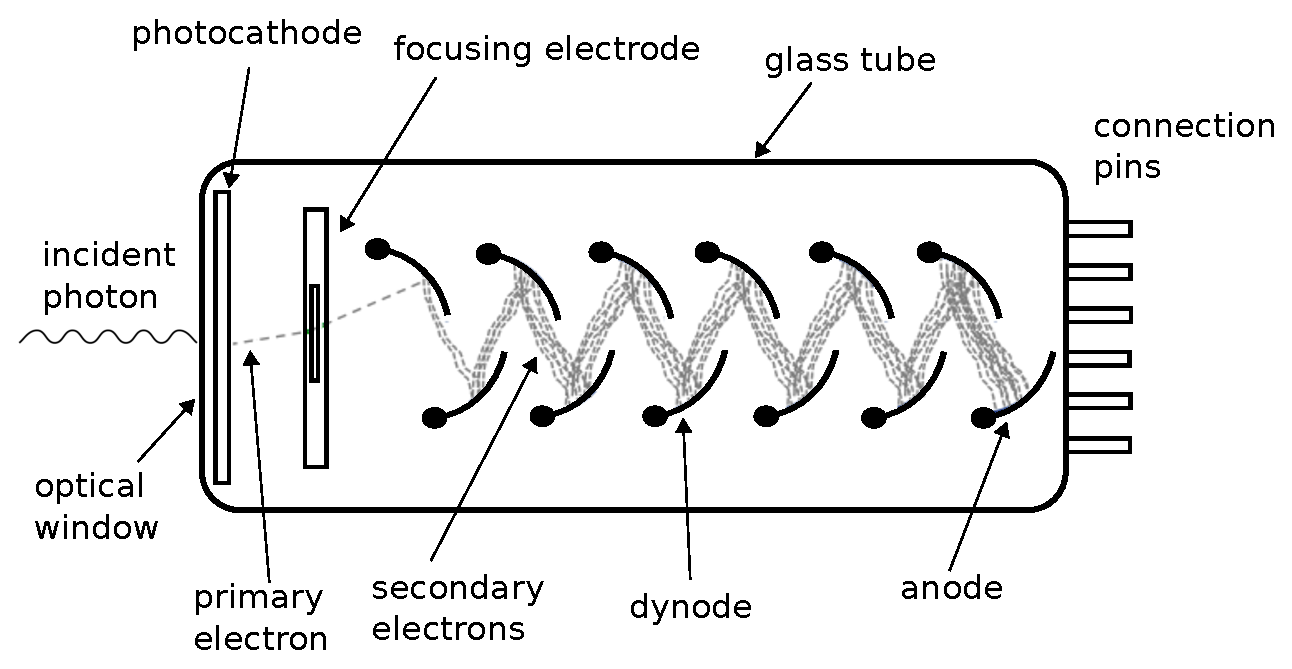
\includegraphics[width=0.5\textwidth]{Figures/PMT.eps}
\caption{PMT functioning sketch. The incident photon impinges the photocathode releasing a primary electron which create a secondary electron avalanche due to the electric field generated along the dynodes. All the PMT parts are encapsulated in a vacuum glass tube.}
\label{Gain_curve}
\end{center}
\end{figure}

A PMT is an optoelectronic device which generates a measurable electric current ($\sim$ mA) by means of photoelectric effect when a photon impinges it. The primary electron knocked away from the photocathode when a photon hits it is subjected to an electrical field created by a potential difference between the dynodes causing than the electron increases its energy pulling up more electrons when it hits the next dynode. This avalanche of secondary electrons along the dynodes is seeming as an amplification of the current that can reach a gain factor of 10$^5$-10$^6$.



We modeled the PMT R5912 taking into account such basic principle of functioning and its intrinsic parameters such as the number of amplification stages and the gain curve. The total gain of the PMT model is defined as:

\begin{equation}
G = \frac{I_a}{I_k}
\end{equation}

where $I_a$ is the anode current and $I_k$ is the photocathode current.

On other hand, PMT gain can be expressed as a function of the gain in each stage, as follows:

\begin{equation}
G =  \beta \prod_{i=1}^{N}  g_i 
\end{equation}

where $g_i$ is the gain in each stage, $N$ in the number of dynodes and $\beta$ is the collection efficiency. The gain $g_i$ depends on the inter-dynode voltage $v_i$, as follows:
%If $ \eta \approx 100\%$, then

\begin{equation}
g_i = k_i v_i^\alpha
\end{equation}

where $k_i$ is a constant and $ 0.6  \leq \alpha \leq 0.8$ is an intrinsic parameter of the PMT. The total gain (2) can be expressed as the product of all the inter-dynode gains or in function of the PMT bias voltage $V_B$ as:

\begin{equation}
G =  \prod_{i=1}^{N}  k_i (V_B \epsilon_i)^{\alpha} 
\end{equation}
where $\epsilon_i$ is the fraction of the bias voltage in each inter-dynode stage as a result of the resistor polarization chain.\\

Taking the asummption of $\epsilon_i = \epsilon$ and $k_i=k_0$, the total gain is expressed as follows:

\begin{equation}
G = k_0^N (V_B \epsilon)^{N\alpha} 
\end{equation}

The last equation describes the behavior of any PMT.

\subsection{Modeling the PMT R5912}


\begin{figure}[h!]
\begin{center}
\includegraphics[width=0.4\textwidth]{Figures/Gain_curve}
\caption{Gain curve of the PMT R5912.The gain of the PMT has an exponential relation depending on the high voltage applied between the anode and cathode, \cite{r5912}.}
\label{Gain_curve}
\end{center}
\end{figure}

In order to get the parameters $\alpha$ and $k_0$ a couple of points $[V_1, G_1]$ and $[V_2, G_2]$ are extracted from the gain versus bias voltage curve of the PMT Hamamatsu R5912 , Fig. \ref{Gain_curve}.\\

The values $[1000 V, 3 \times 10^5 ]$ and $[1500 V, 7 \times 10^6]$ were chosen. A pair of equations are derived from (5) for the given points in order to solve the unknown quantifies ($\alpha$, $k_0$).

\begin{equation}
G1 = k_0^N (V_1 \epsilon)^{N \alpha}
\end{equation}

\begin{equation}
G2 = k_0^N (V_2 \epsilon)^{N \alpha}
\end{equation}

where the number of dynodes is $N=10$. In the same way, the parameter $\epsilon$ is calculated by means of the voltage distribution ratio in the resistive polarization chain which is provided for the PMT datasheet, Fig. \ref{Chain}.

\begin{table}[ht]
\centering
  \caption{ Tapered voltage distribution for linear measurement}
  \begin{tabular}{ | c | c |}
    \hline
    Electrodes & Ratio, $R_i$  \\ \hline
    K-Dy1 & 11.3  \\ \hline
    Dy1-F2 & 0  \\ \hline
    F2-F1 &  0.6 \\ \hline
    F1-F3 & 0 \\ \hline
    F3-Dy2 & 3.4 \\ \hline
    Dy2-Dy3 & 5 \\ \hline
    Dy3-Dy4 & 3.33 \\ \hline
    Dy4-Dy5 & 1.67  \\ \hline
    Dy5-Dy6 & 1  \\ \hline
    Dy6-Dy7 & 1.2  \\ \hline
    Dy7-Dy8 & 1.5  \\ \hline
    Dy8-Dy9 & 2.2  \\ \hline
    Dy9-Dy10 & 3  \\ \hline
    Dy10-P & 2.4  \\
    \hline
  \end{tabular}
  \label{net}
\end{table}

In this case, a linear behavior of the PMT is desired, for this reason, the tapered voltage distribution was chosen. The condition for determining the $\epsilon$ value is
\begin{equation}
\epsilon  \sum_i R_i = 1
\end{equation}
where $R_i$ is the ratio in each inter-electrode stage $i$. Therefore, the estimated $\epsilon$ value is 0.02732.\\

Then, an expression for $k_0$ is obtain from (7) as follows

\begin{equation}
k_0=\sqrt[N]{\frac{G_2}{(V_2\epsilon)^{N \alpha}}}
\end{equation}
Replacing (9) in (6) the parameter $\alpha$ is defined as:

\begin{equation}
\alpha=\frac{\log \left( \frac{G_1}{G_2} \right)}{N \log \left( \frac{V_1}{V_2} \right)}
\end{equation}
From (9) and (10) $k_0=0.27$ and $\alpha= 0.7768$ are obtained.


\subsection{PMT and passive biasing network Spice simulation}

The dynodes and anode currents were modeled as function of the parameters $k_0$, $\alpha$ , $\epsilon$, $V_B$ and $N$. The current flowing through $i^{th}$ dynode is defined as follows:

\begin{equation}
Id_{i} = I_k \frac{k_0^N (V_B \epsilon)^{N \alpha}}{(k_0 (v_i \epsilon)^\alpha)^{N+1-i}}, \ \ \ i=1,2, \cdots N
\label{Id}
\end{equation}

The anode current is:
\begin{equation}
Ia = I_k k_0^N (V_B \epsilon)^{N \alpha}
\label{Ia}
\end{equation}

The PMT and its biasing network were simulated using the Orcad Pspice software. We used the GVALUE  \cite{Krihely2014} block for modeling the PMT currents flowing along each PMT dynode from the cathode to the anode. This block sets the transfer function described by the equations \ref{Id} and \ref{Ia} for each amplification stage depending on the voltage applied between adjacent dynodes. 

\begin{figure}[h!]
\begin{center}
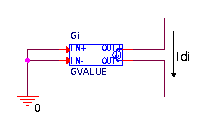
\includegraphics[width=0.35\textwidth]{Figures/GVALUE}
\caption{Elemental gain block used to simulate the inter-dynode stages.}
\label{Gval}
\end{center}
\end{figure}

Resistive divider networks are the most widely used method to bias PMTs \cite{Camin1999PassiveAA}. In order to reduce the non linearity of the PMT response due to space-charge effect we selected a tapered resistive chain and to use decopling capacitors \cite{Huang_2013}. The resistor values were estimated taking into account the datasheet recommendation of the interdynode ratios presented in the Table \ref{net}. 

Decoupling capacitors of 20 nF were connected from the dynode d5 to the anode. The connection between decoupling capacitors is serial and parallel. On the other hand, we filter DC components of the outputs at the anode and last dynode using coupling capacitors of 4.7 nF. For avoiding oscillations in the signal due to reflections by bad impedance coupling during the transmission to the electronics readout we implemented 50 $\Omega$ loads at the outputs. 

An amplification stage was connected to the last dynode output in order to have two readable outputs and for increasing the measurable range. When the ADC connected to the amplified dynode is saturated because the pulse amplitude exceeds its range, we read the anode output searching for a complete shaped pulse from which we can obtain clean information. This dynode amplification is around 20 times.

In Fig. \ref{Circuit} the complete schema of the Spice model is shown.


\begin{figure}[h!]
\begin{center}
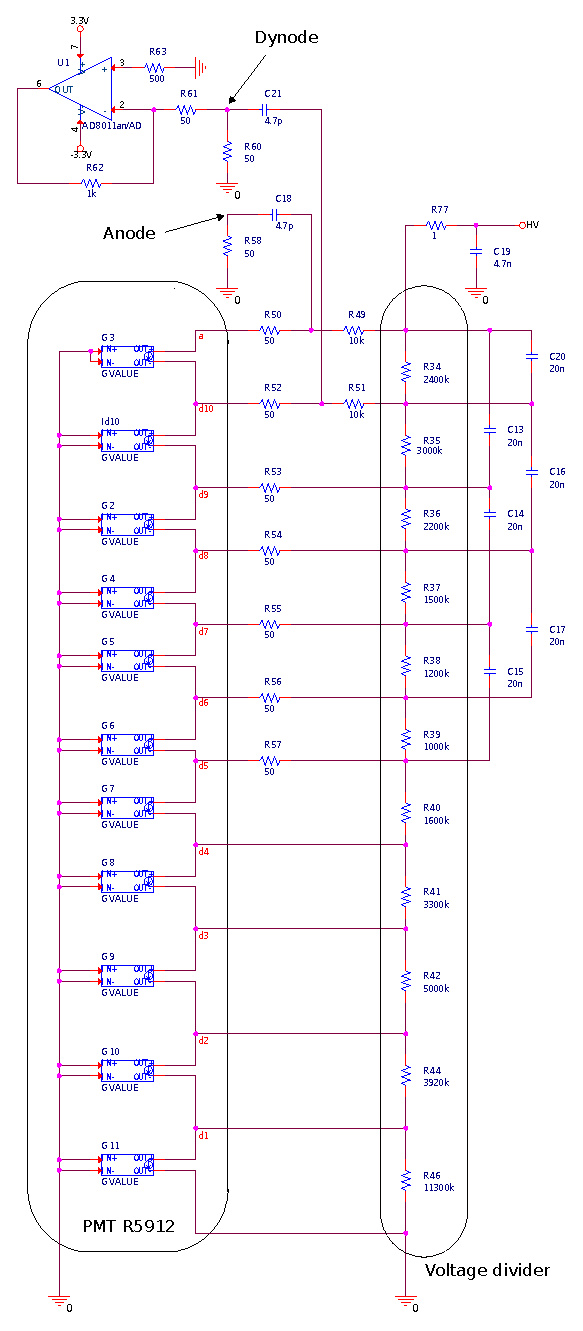
\includegraphics[width=0.45\textwidth]{Figures/Circuit}
\caption{Spice model for the PMT R5912 and its resistive polarization chain.}
\label{Circuit}
\end{center}
\end{figure}






\subsection{Incident photon yield and cathode current}

Simulations using the particle-matter interaction code GEANT4 were carried out for modeling the incident photon pulse on the PMT when charged particles pass along the WCD. We injected 10$^5$ muons with 3 GeV energy perpendicularly to a 120 cm height WCD. The average number of Cherenkov photons $N_{\gamma}$ generated along the path were 46857, however only 1617 of such photons reach the optical window of the PMT and around 203.2 photoelectrons $N_{pe}$ were produced in the photocathode due to the quantum efficiency $\eta$ of the PMT R5912. In this case, the maximum $\eta = 22 \%$ (at 390 nm) was taking into account. Then, the number of photo-electrons is

\begin{equation}
N_{pe} = \eta N_{\gamma}
\end{equation}

The number of photoelectrons depending on the arrival time of the incident photons is shown in Fig. \ref{pulse_G4}. The pulse is attenuated following a decreasing exponential tendency with an attenuation time of  42.12 ns and a time extension up 250 ns.

\begin{figure}[h!]
\begin{center}
\includegraphics[width=0.5\textwidth]{Figures/pulse_vem.png}
\caption{Simulation of the Cherenkov photons number in the Chitaga WCD for a muon of 1 GeV (green line) and 10 GeV (red line). }
\label{pulse_G4}
\end{center}
\end{figure}

%The figure shows the number of cherenkov photons $N_{\gamma}$ hitting the PMT surface during a short period of time. In order to calculate the number of photo-electrons $N_{pe}$ generated by photoelectric effect in the PMT cathode is necessary introduce the quantum efficiency Q.E. of the PMT, Fig. \ref{QE}.

% \begin{figure}[h!]
% \begin{center}
% \includegraphics[width=0.4\textwidth]{Figures/QE}
% \caption{Quantum efficiency for the PMT R5912.}
% \label{QE}
% \end{center}
% \end{figure}

On the another hand, the electric charge in the cathode is calculated as

\begin{equation}
Q = N_{pe}*e
\end{equation}
where $e$ is the electron charge ($1.6 \time 10^{-19}$ Coulombs). Finally, the cathode current $I_k$ is estimated as follows

\begin{equation}
I_k = \frac{Q}{t}
\end{equation}

\begin{figure}[h!]
\begin{center}
\includegraphics[width=0.5\textwidth]{Figures/Cathode_current}
\caption{Cathode current source taking into account the quantum efficiency and the number of Cherenkov photons for a muon of 1 GeV.}
\label{cathode}
\end{center}
\end{figure}

In Fig. \ref{cathode} the estimated cathode current when a 3 GeV vertical muon impinges the WCD is shown. The maximum peak of the current is roughly 17 nA which can generate a 17 mA anode current setting a PMT gain of 10$^6$.

\section{RESULTS}

\subsection{Vertical muon charge}

The PMT bias was set to 1000 V which means a gain 2.9$\times$10$^5$, if a vertical muon hits the WCD a current signal of $\sim$ 5 mA is measured at the PMT anode. A voltage pulse 250 mV amplitude appears across the 50 $\Omega$ load at the anode output. Such pulse is digitized at 40 MHz (25 ns step) in a 12 samples vector with a relation UADC $\approx$ 1 mV as is shown in Fig. \ref{digitized}. The pulse charge (area under curve) for the simulated vertical muon is 321.6 ADC.Bin which is 4$\%$ less than the real value obtained from measurements (333 ADC.bin).


\begin{figure}[h!]
\begin{center}
\includegraphics[width=0.5\textwidth]{Figures/dig_pulse.png}
\caption{Gain curve obtained from the Spice simulation.}
\label{digitized}
\end{center}
\end{figure}


\subsection{Response of the PMT and bias chain model}

\begin{figure}[h!]
\begin{center}
\includegraphics[width=0.5\textwidth]{Figures/spice_pulse.png}
\caption{Gain curve obtained from the Spice simulation.}
\label{QE}
\end{center}
\end{figure}

% \begin{figure}[h!]
% \begin{center}
% \includegraphics[width=0.35\textwidth]{Figures/Gain_model}
% \caption{Gain curve obtained from the Spice simulation.}
% \label{QE}
% \end{center}
% \end{figure}

\subsection{Linearity}




\begin{figure}[h!]
\begin{center}
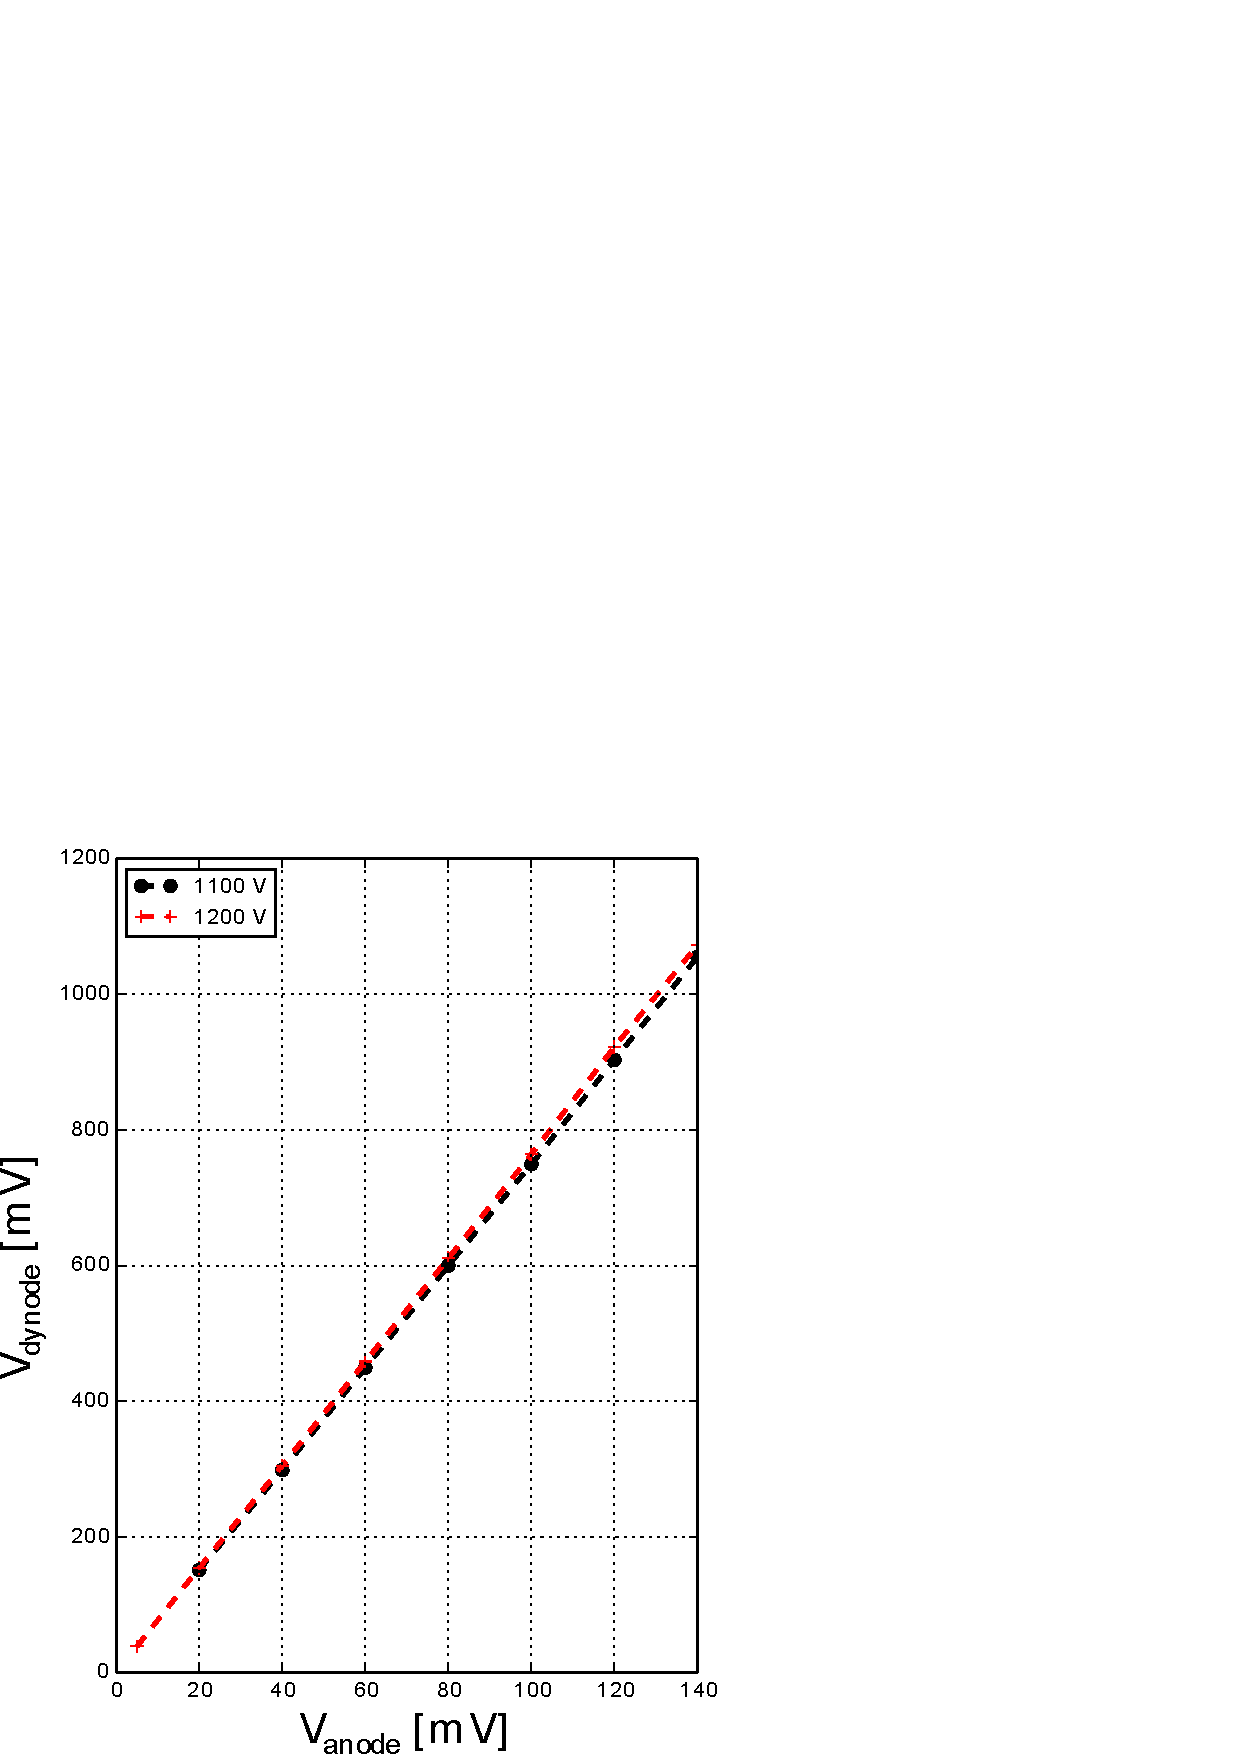
\includegraphics[width=0.35\textwidth]{Figures/Linear.png}
\caption{Gain curve obtained from the Spice simulation.}
\label{QE}
\end{center}
\end{figure}

\subsection{Simulation and data comparison}

\begin{figure}[h!]
\begin{center}
\includegraphics[width=0.5\textwidth]{Figures/Base.eps}
\caption{Elemental gain block used to simulate the inter-dynode stages.}
\label{Chain}
\end{center}
\end{figure}

\begin{figure}[h!]
\begin{center}
\includegraphics[width=0.35\textwidth]{Figures/Fit_1100}
\caption{The general structure.}
\label{QE}
\end{center}
\end{figure}

\begin{figure}[h!]
\begin{center}
\includegraphics[width=0.35\textwidth]{Figures/Fit_1200}
\caption{Comparison between the spice model and the data acquired by the Chitaga WCD.}
\label{QE}
\end{center}
\end{figure}



Comparación entre la amplitud dínodo y ánodo cambiando de voltaje HV en la simulación y datos de la base diseñada.

Linealidad del PMT

Ref. Design of the photomultiplier bases for the surface detectors of the Pierre Auger Observatory
\section{CONCLUSIONS}


\addtolength{\textheight}{-12cm}   % This command serves to balance the column lengths
                                  % on the last page of the document manually. It shortens
                                  % the textheight of the last page by a suitable amount.
                                  % This command does not take effect until the next page
                                  % so it should come on the page before the last. Make
                                  % sure that you do not shorten the textheight too much.

%%%%%%%%%%%%%%%%%%%%%%%%%%%%%%%%%%%%%%%%%%%%%%%%%%%%%%%%%%%%%%%%%%%%%%%%%%%%%%%%



%%%%%%%%%%%%%%%%%%%%%%%%%%%%%%%%%%%%%%%%%%%%%%%%%%%%%%%%%%%%%%%%%%%%%%%%%%%%%%%%



%%%%%%%%%%%%%%%%%%%%%%%%%%%%%%%%%%%%%%%%%%%%%%%%%%%%%%%%%%%%%%%%%%%%%%%%%%%%%%%%
% \section*{APPENDIX}

% Appendixes should appear before the acknowledgment.

\section*{ACKNOWLEDGMENT}

This work was developed at Halley Research Group at Universidad Industrial de Santander.



\bibliographystyle{unsrt}
\bibliography{LAGO.bib}



\end{document}
